\documentclass[language=german,style=solution]{smo}
\examtime{4 Stunden}
\place{1./2. Prüfung}
\examdate{13./14. März 2015}

\usepackage{tikz}

\title{SMO - Finalrunde Musterlösung}

\begin{document}

\begin{enumerate}

\item[\textbf{1.}] Sei $ABC$ ein spitzwinkliges Dreieck mit $AB\neq BC$ und Umkreis $k$. Seien $P$ und $Q$ die Schnittpunkte von $k$ mit der Winkelhalbierenden beziehungsweise der Aussenwinkelhalbierenden von $\angle CBA$. Sei $D$ der Schnittpunkt von $AC$ und $PQ$. Bestimme das Verhältnis $AD:DC$.

\textbf{1 ère solution:}\\
Par le théorème de l'angle inscrit et le fait que $BP$ est la bissectrice de $\angle ABC$, $\angle PCA = \angle PBA = \angle PBC = \angle PAC$, donc $\triangle APC$ est isocèle. De même, prenons $R$ un point sur la droite $AB$ tel que $B$ est entre $A$ et $R$. Alors $\angle QAC = \angle QBC = \angle QBR = 180^\circ - \angle QBA = \angle QCA$, où nous avons utilisé le fait que $QB$ est la bissectrice extérieure de $\angle ABC$ et le fait que $ABQC$ est un quadrilatère inscrit. Ainsi $\triangle AQC$ est aussi un triangle isocèle. Comme $P$ et $Q$ sont tous les deux à égale distance de $A$ et $C$, donc $PQ$ est la médiatrice de $AC$, ce qui signifie que $D$ est le milieu du segment $AC$. Nous obtenons donc que $\frac{AD}{DC} = 1$.

\textbf{2ème solution:}\\
On démontre comme ci-dessus que $\triangle AQC$ est isocèle en $Q$. De plus, $\angle CQP = \angle CBP = \angle ABP = \angle AQP$, où nous utilisons le théorème de l'angle inscrit et le fait que $BP$ est la bissectrice intérieure de $\angle ABC$. Ainsi $QD$ est la bissectrice de $\angle AQC$ est donc comme le triangle est isocèle $QD$ est la médiatrice de $AB$. On conclut donc que $\frac{AD}{DC} = 1$.

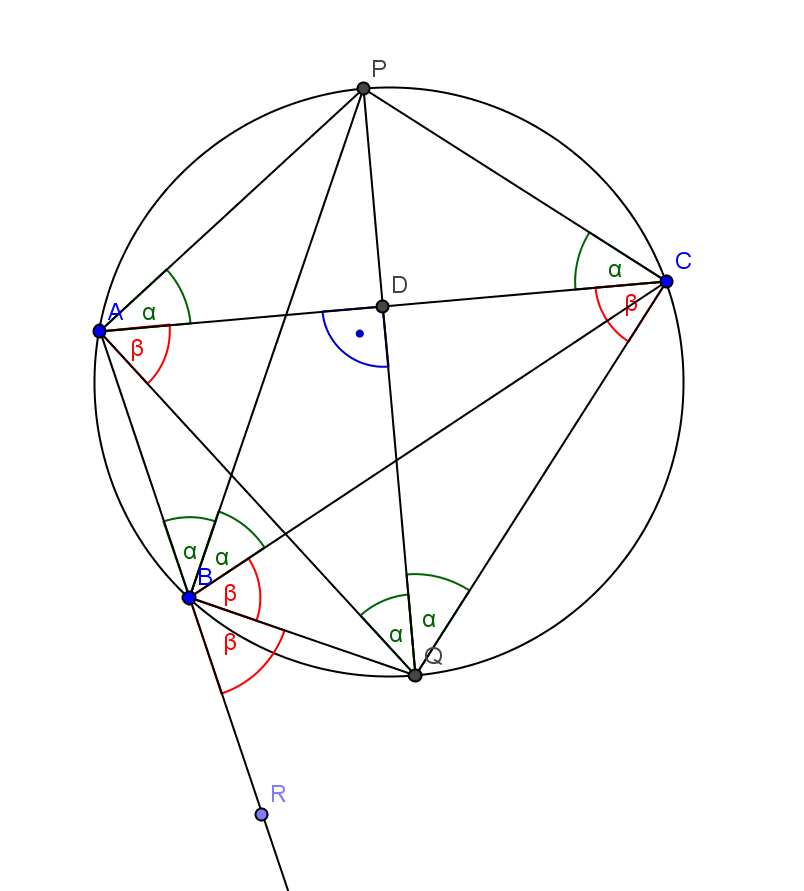
\includegraphics{Finalrunde_1}

\newpage

\item[\textbf{2.}] Bestimme alle Paare $(m,p)$ natürlicher Zahlen, sodass $p$ eine Primzahl und
\[2^mp^2+27 \]
die dritte Potenz einer natürlichen Zahl ist.

\textbf{Lösung} Die dritte Potenz $n^3$ ist ungerade, also auch $n$. Umformen führt zu
\[
2^mp^2=n^3-3^3
\]
Die rechte Seite kann man ausklammern als
\[
2^mp^2=(n-3) (n^2+3n+9).
\]
Der zweite Faktor ist ungerade, folglich gilt $2^m \div (n-3)$. Ausserdem gilt $p^2 \div (n^3+3n+9)$, denn $n^3+3n+9$ ist grösser als $n-3$. Nun liegt der zweite Faktor zwischen $(n+1)^2$ und $(n+3)^2$. Da der Faktor selbst ein Quadrat ist, gilt $p^2=(n+2)^2$. Also erhalten wir $n^2+3n+9=n^2+4n+4$, was zu $n=5$ führt. Folglich ist $2^m=2$, also $m=1$ sowie $p^2=49$. Die einzige Lösung ist somit $(1,7)$.

\newpage

\item[\textbf{3.}] Finde alle Funktionen $f: \R \to \R$, sodass für alle $x,y \in \R$ gilt:
\[
(y+1)f(x) + f(xf(y)+f(x+y))=y.
\]

\textbf{Solution:} Soit $(y+1)f(x)+f(xf(y)+f(x+y))=y$.
On remarque que $f(x)\equiv 1$ n'est pas une solution. Donc il existe $x_0$ tel que $f(x_0)\neq 1$.
En substituant $x=x_0$, on obtient :
\[
	f(x_0f(y)+f(x_0+y))=y(1-f(x_0))-f(x_0)
\]
Cette égalité montre que $f$ est surjective. En effet, on a un terme fonctionnel en $y$ à gauche et une fonction affine (donc surjective) à droite.\\
Ainsi, il existe $a$ tel que $f(a)=0$. En substituant $x=0,y=a$, on obtient :
\[
	f(0)(a+2)=a
\]
On en conclue que $f(0)\neq 1$.\\
Substituons maintenant $x=0$ dans la première équation pour obtenir :
\[
	f(f(y))=y(1-f(0))-f(0)
\]
Cette équation montre que $f$ est injective. En effet, si on prend $u$ et $v$ tels que $f(u)=f(v)$, alors :
\[
	u(1-f(0))-f(0)=f(f(u))=f(f(v))=v(1-f(0))-f(0) \Rightarrow u=v
\]
Substituons $x=a,y=0$ dans l'équation de départ pour obtenir : 
\[
	f(af(0))=0=f(a) \Rightarrow af(0)=a \Rightarrow a=0 \Rightarrow f(0)=0
\]
La première implication découle de l'injectivité et la deuxième du fait que $f(0)\neq 1$.\\
Substituons finalement $x=0$, puis $y=0$ et on a :
\[
	f(f(y))=y \text{ et } f(f(x))=-f(x)
\]
On en conclue que $f(x)\equiv -x$, dont on vérifie facilement que c'est bien une solution.

\newpage

\item[\textbf{4.}] Gegeben seien ein Kreis $k$ und zwei Punkte $A$ und $B$ ausserhalb des Kreises. Gib an, wie man mit Zirkel und Lineal einen Kreis $\ell$ konstruieren kann, sodass $A$ und $B$ auf $\ell$ liegen und sich $k$ und $\ell$ berühren.

\textbf{Lösung} Als Erstes konstruieren wir die Mittelsenkrechte $m$ der Strecke $AB$. Sei $O$ der Mittelpunkt von $k$. Falls $O$ auf $m$ liegt, dann wählen wir einen der beiden Schnittpunkte von $m$ mit $k$ und nennen ihn $P$. Wir können $P$ immer so wählen, dass $A$, $B$ und $P$ nicht auf einer Geraden liegen. Konstruiere nun den Kreis $\ell$ durch die Punkte $A$, $B$ und $P$, und nenne seinen Mittelpunkt $M$. Da der Punkt $P$ auf beiden Kreisen liegt und gleichzeitig auch auf $m$, also der Geraden durch die beiden Mittelpunkte dieser Kreise, können wir folgern, dass sich die Kreise $k$ und $\ell$ berühren. Somit erfüllt $\ell$ die gewünschten Bedingungen.\\
Nehme nun an, der Punkt $O$ liege nicht auf $m$. Wähle einen beliebigen Punkt $P$ auf $k$, der nicht auf der Geraden $AB$ liegt, und konstruiere den Kreis $h$ durch die Punkte $A$, $B$ und $P$. Falls sich $k$ und $h$ berühren, wählen wir $\ell=h$ und sind fertig. Wenn dies nicht der Fall ist, gibt es einen weiteren Schnittpunkt $Q$ von $k$ und $h$. Betrachte nun die Geraden $AB$ und $PQ$. Wir wollen zeigen, dass diese Geraden nicht parallel sein können. Nehme also an, $AB$ und $PQ$ seien parallel. Da die Strecken $AB$ und $PQ$ beides Sehnen im Kreis $h$ sind, folgt daraus, dass die Mittelsenkrechten dieser beiden Strecken übereinstimmen. $PQ$ ist gleichzeitig auch eine Sehne im Kreis $k$, und somit liegt $O$ auf dieser gemeinsamen Mittelsenkrechten, die aber gerade $m$ ist. Dies ist ein Widerspruch, da wir angenommen haben, dass $O$ nicht auf $m$ liegt.\\
Wir haben nun gezeigt, dass $AB$ und $PQ$ nicht parallel sind, und somit gibt es einen Schnittpunkt $S$. Konstruiere nun eine Tangente durch den Punkt $S$ an den Kreis $k$ und nenne den Berührungspunkt $T$. $PQ$ ist die Potenzlinie der Kreise $k$ und $h$, also gilt:
\[
SA\cdot SB=SP\cdot SQ=ST^2.
\]
Nach der Umkehrung des Potenzsatzes folgt hieraus, dass die Gerade $ST$ eine Tangente an den Umkreis des Dreiecks $ABT$ ist. Konstruiere diesen Kreis und nenne ihn $\ell$. Da $ST$ auch eine Tangente an den Kreis $k$ ist, bedeutet dies, dass sich $k$ und $\ell$ im Punkt $T$ berühren, und wir sind fertig.

\textit{Marking Scheme:} Für die Angabe einer richtigen Konstruktion im Fall, dass $O$ auf der Mittelsenkrechten von $AB$ liegt, gibt es 1 Punkt. Für den allgemeinen Fall gibt es 6 Punkte, wobei bis zu zwei Punkte abgezogen werden können, falls mögliche Probleme nicht beachtet werden (z.B. wenn man den Schnittpunkt zweier paralleler Geraden definiert oder den Umkreis dreier Punkte, die auf einer Geraden liegen).

\newpage

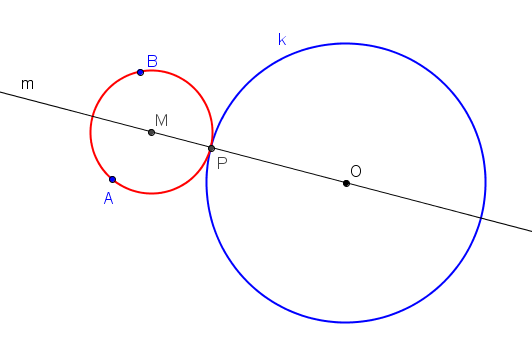
\includegraphics{Finalrunde4_1}

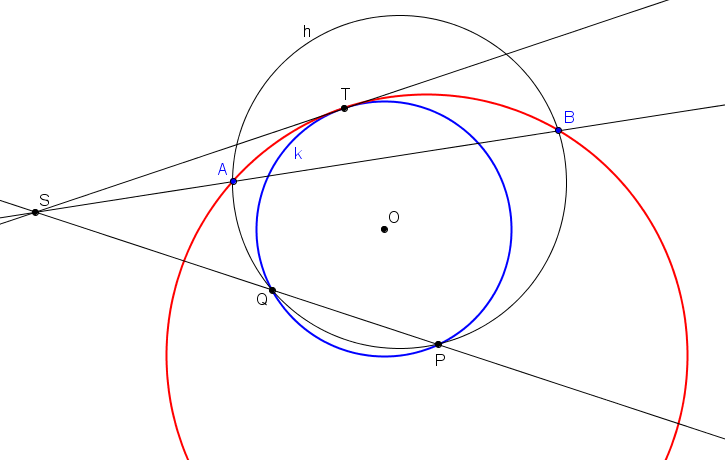
\includegraphics{Finalrunde4_2}

\newpage

\item[\textbf{5.}] Sei $m$ eine natürliche Zahl. Auf der SMO-Wandtafel steht $2^m$ mal die Zahl $1$. In einem Schritt wählen wir zwei Zahlen $a$ und $b$ auf der Tafel und ersetzen sie beide jeweils durch $a+b$.\\
Zeige, dass nach $m2^{m-1}$ Schritten die Summe der Zahlen mindestens $4^m$ beträgt.

\textbf{Lösung:} Sei $S$ die Summe der Zahlen nach $m2^{m-1}$ Zügen. Die Idee ist, zuerst eine untere Schranke für das Produkt der $2^m$ Zahlen zu finden. Sei dazu $P_i$ das Produkt aller Zahlen nach dem $i$-ten Schritt und $P_0 = 1$. In jedem Schritt werden zwei Zahlen $a,b$ durch $a+b,a+b$ ersetzt. Deren Produkt ändert sich von $ab$ zu $(a+b)^2 \geq 4ab$. Daraus folgt direkt $P_{i+1} \geq 4P_i$ und somit $P_{m2^{m-1}} \geq $. Mit AM-GM folgt nun
\[ S \geq 2^{m}(4^{m2^{m-1}})^\frac{1}{2^m} = 4^m,\]
was zu zeigen war.

\textit{Marking Scheme:} Bei dieser Aufgabe kann man im Wesentlichen $0$ oder $7$ Punkte erreichen. Einen Punkt kann man erhalten, falls man bemerkt, dass sich das Produkt der zwei Zahlen, die man in einem Zug verändert mindestens um einen Faktor 4 grösser wird.

\newpage

\item[\textbf{6.}] 
Wir haben ein $8 \times 8$ Brett. Eine \emph{innere Kante} ist eine Kante zwischen zwei $1 \times 1$ Feldern. Wir zerschneiden das Brett in $1 \times 2$ Dominosteine. Für eine innere Kante $k$ bezeichnet $N(k)$ die Anzahl Möglichkeiten, das Brett so zu zerschneiden, dass entlang der Kante $k$ geschnitten wird. Berechne die letzte Ziffer der Summe, die wir erhalten, wenn wir alle $N(k)$ addieren, wobei $k$ eine innere Kante ist.

\textbf{Lösung:} Zuerst berechnen wir, entlang wie vielen inneren Kanten bei einer Zerlegung geschnitten wird. Insgesamt gibt es je $7 \cdot 8$ horizontale und vertikale innere Kanten. Bei einer Zerlegung wird das Brett entlang allen inneren Kanten, ausser den $32$ innerhalb eines Dominosteines, geschnitten. Somit wird bei jeder Zerlegung entlang von $2 \cdot (7 \cdot 8) - 32 = 80$ inneren Kanten geschnitten. Dies heisst, dass jede Zerlegung $80$ mal gezählt wird. Somit wissen wir, dass die Summe aller $N(k)$ durch $80$ teilbar ist. Daraus folgt, dass die letzte Ziffer der Summe null ist. 

\newpage

\item[\textbf{7.}] Seien $a,b,c$ reelle Zahlen, sodass gilt:
\[
\frac{a}{b+c}+\frac{b}{c+a}+\frac{c}{a+b} = 1.
\]
Bestimme alle Werte, welche folgender Ausdruck annehmen kann:
\[
\frac{a^2}{b+c}+\frac{b^2}{c+a}+\frac{c^2}{a+b}.
\]

\textbf{Lösung:}

\begin{align*}
a+b+c &= a+b+c\\
\overbrace{\left( \frac{a}{b+c}+\frac{b}{a+c}+\frac{c}{a+b}\right)}^{1} \cdot (a+b+c) &=a+b+c\\
\frac{a^2}{b+c}+\frac{a(b+c)}{b+c}+\frac{b^2}{a+c}+\frac{b(a+c)}{a+c}+\frac{c^2}{a+b}+\frac{c(a+b)}{a+b}&=a+b+c\\
\frac{a^2}{b+c}+\frac{b^2}{a+c}+\frac{c^2}{a+b}+a+b+c &= a+b+c\\
\frac{a^2}{b+c}+\frac{b^2}{a+c}+\frac{c^2}{a+b} &= 0
\end{align*}

\newpage

\item[\textbf{8.}] Sei $ABCD$ ein Trapez, wobei $AB$ und $CD$ parallel sind. $P$ sei ein Punkt auf der Seite $BC$. Zeige, dass sich die Parallelen zu $AP$ und $PD$ durch $C$ respektive $B$ auf $DA$ schneiden.

\textbf{Lösung:} Sei $X$ der Schnittpunkt von $DA$ und der Parallelen zu $AP$ durch $C$ und sei $Y$ der Schnittpunkt von $DA$ und der Parallelen zu $PD$ durch $B$. Wir betrachten zuerst den Fall, dass $BC$ und $DA$ parallel sind. Dann ist $ABCD$ ein Parallelogramm und eine Punktspiegelung am Diagonalenschnittpunkt führt $ABCD$ in sich selbst über. Betrachte den Bildpunkt $P'$ von $P$ auf der Seite $DA$. Die Gerade $AP$ wird bei der Punktspiegelung auf die Gerade $CP'$ abgebildet. Das bedeutet aber, dass $CP'$ parallel zu $AP$ ist, folglich ist $CP'$ gerade die Parallele zu $AP$ durch $C$ und es gilt $X=P'$. Analog zeigen wir $Y=P'$, was diesen Fall abschliesst.\\
Nehme nun an, die Geraden $BC$ und $DA$ seien nicht parallel und bezeichne ihren Schnittpunkt mit $T$. Dann gilt nach dem Strahlensatz:
\[
\frac{TA}{TX}=\frac{TP}{TC},\;\;\frac{TB}{TP}=\frac{TY}{TD}\;\;\text{und}\;\;\frac{TA}{TB}=\frac{TD}{TC}.
\]
Hieraus folgt:
\[
\frac{TY}{TX}=\frac{TB\cdot TD}{TP}\cdot\frac{TP}{TA\cdot TC}=1. 
\]
Somit gilt $TX=TY$, woraus $X=Y$ folgt.

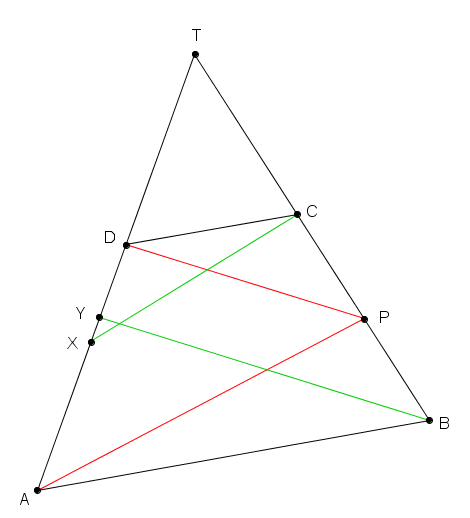
\includegraphics{Finalrunde_8}
\newpage

\item[\textbf{9.}] Sei $p$ eine ungerade Primzahl. Bestimme die Anzahl Tupel $(a_1,a_2,\dots,a_p)$ natürlicher Zahlen mit folgenden Eigenschaften:
\begin{enumerate}[1)]
\item $1\leq a_i\leq p$ für alle $i=1,\dots,p$.
\item $a_1+a_2+\dots +a_p$ ist nicht durch $p$ teilbar.
\item $a_1a_2 + a_2a_3 +\dots a_{p-1}a_p + a_pa_1$ ist durch $p$ teilbar.
\end{enumerate}

\textbf{Lösung:} Für ein Tupel $t=(a_1,\dots,a_p)$ wir in 1) definieren wir $S(t) = a_1+\dots +a_p$ und $P(t) = a_1a_2+a_2a_3+\dots +a_pa_1$. Wir halten fest
\[
\abs{\{t \ | \ t \text{ erfüllt 1 und 2}} = p^{p-1}(p-1),
\]
da wir die ersten $p-1$ Einträge frei wählen können und dann genau ein Wert für den letzten Eintrag verboten ist.\\
Wir definieren weiter für $0\leq k \leq p-1$ ein neues Tupel $t_k =(a_1+k,a_2+k,\dots,a_p+k)$, wobei wir im Fall, dass einer der Einträge grösser als $p$ ist, diesen durch seinen Rest bei Division durch $p$ ersetzen. \\
Es gilt $S(t_k) \equiv S(t) (\text{ mod }p)$ und $P(t_k) \equiv P(t) + 2kS(t) (\text{ mod }n)$. Sei nun $t$ ein Tupel, welches $1$ und $2$ erfüllt. Dann durchläuft $2kS(t)$ für $0\leq k\leq p-1$ jede Restklasse modulo $p$ genau einmal und somit erfüllt genau eines der Tupel $t_0,t_1,\dots,t_{p-1}$ zusätzlich $3$. Somit ist die gesuchte Anzahl gleich
\[
\abs{\{t \ | \ t \text{ erfüllt 1 und 2\}}}{p}= \frac{p^{p-1}(p-1)}{p}= p^{p-2}(p-1).
\]

\newpage

\item[\textbf{10.}] Finde die grösste natürliche Zahl $n$, sodass für alle reellen Zahlen $a,b,c,d$ folgendes gilt:
\[
(n+2) \sqrt{a^2+b^2} + (n+1) \sqrt{a^2+c^2} + (n+1)\sqrt{a^2+d^2} \geq n(a+b+c+d).
\]

\textbf{Solution:} L'idée est d'appliquer Cauchy-Schwarz sur les trois racines de gauche :
\begin{align*}
&(n+2)\sqrt{a^2+b^2}+(n+1)\sqrt{a^2+c^2}+(n+1)\sqrt{a^2+d^2}\\
= &\sqrt{(4n+4)+n^2}\sqrt{a^2+b^2}+\sqrt{(2n+1)+n^2}\sqrt{a^2+c^2}+\sqrt{(2n+1)+n^2}\sqrt{a^2+d^2}\\
\geq &(2a\sqrt{n+1}+nb)+(a\sqrt{2n+1}+nc)+(a\sqrt{2n+1}+nd)\\
= & a(2\sqrt{n+1}+2\sqrt{2n+1})+n(b+c+d)
\end{align*}

Pour les trois inégalités que nous avons appliquées il y a, par exemple, le cas d'égalité suivant 
\[
	(a,b,c,d)=(1,\frac{n}{2\sqrt{n+1}},\frac{n}{\sqrt{2n+1}},\frac{n}{\sqrt{2n+1}})
\]
qui en remplaçant dans l'inégalité de départ nous donne la condition nécessaire :
\[
	2(\sqrt{n+1}+\sqrt{2n+1})\geq n
\]
En élevant deux fois au carré et en simplifiant on obtient $n \leq 24$ avec égalité si $n=24$. Donc $n=24$ est bien la valeur optimale.

\end{enumerate}

\end{document}
